%!TEX root = ../../main.tex

\section{Flowsensor}
Til kontrol at vandflow til systemet, er valgt at benytte en flow sensor af typen YF S201. 
Dette er en Hall Effect sensor. En Hall Effekt sensor benytter ændringer i et nær-magnetfelt til at 
ændre sensorens outputspænding, dette genererer et PWM-output der identificerer den mængde vand 
der flyder igennem sensoren, og kan omregnes til mængde vand pr. enhed.

Flowraten udregnes efter formlen: 
				
\begin{figure}[H]
    \begin{align*}
       \frac{Pulse frequency [Hz]}{7.5} = flowrate[L/min]
    \end{align*}
\label{eq:PWM}
\caption{Beregning af flowrate}
\end{figure}				

Ved denne udregning svarer eks. $16Hz = 2L/min, og 65.5HZ = 8L/min$. \newline
Denne måde at beregne flowet på giver i midlertidig problemer med implementering på KarPSoC'en, da dette ville kræve at programmet "lagde beslag" på processoren for at udregne flowet over en given tid. Da KarPSoC-programmet har til formål at køre adskillige opgaver vedrørende Karret, er det ganske enkelt ikke en mulighed at følge denne implementering.\newline
En alternativ implementering blev valgt for at imødekommende denne problematik. Ved praktisk at måle den mængde vand pr. antal PWM-cycle der flyder igennem sensoren, er det muligt at opstille en model for hvor meget vand der flyder til karret baseret på det antal PWM-cycles der modtages af programmet.\newline
Flowsensoren tilkobles via 3 medfølgende pins.

\begin{figure}[H]
	\begin{center}
		\begin{tabular}{ l l }
			 \textcolor{black}{Sort}:   & $GND(-)$ 		\\ 
			 \textcolor{yellow}{Gul}:   & $PWM output$ 	\\  
			 \textcolor{red}{Red}:    	& $VCC(+5V)$ 	\\
		\end{tabular}
	\end{center}
\caption{Pinoversigt}
\end{figure}

Output fra sensoren følger CMOS-standarden, det vil sige at den kan kobles direkte til en given inputpin på PSoC'en. Output-raten gives som udgangspunkt med en målepræcision på +/- 10%.
 
Under operation sinker sensoren 15mA, derved kan den kan trække sin forsyning direkte fra PSoC'en.

\subsection{Counter-kredsløb}
For at aflaste Kar-PSoC'en der håndtere flowsensoren, designes et eksternt counter-kredsløb. Herved minimeres det antal interrupts der trækkes på PSoC-programmet. Kredsløbet designes ved brug af en 4-bit counter (74HC393) samt en 2-input AND-gate (74HC08). 
Kredsløbet er koblet således at PWM-output fra flowsensoren kobles til clock-input 1 (CP1) på counter'en. Outputs fra denne (Q1, Q3) kobles til AND'gaten.
Kredsløbet ses på \ref{screenshot:counter} herunder. 

\begin{figure}[H]
	\centering
	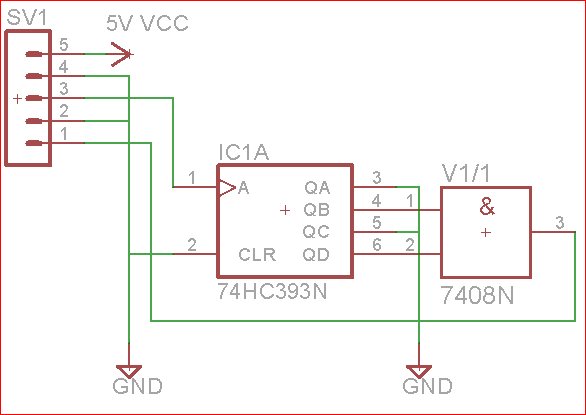
\includegraphics[height=5cm]{../Hardware/Flow_Sensor/Screenshots/FlowSensor_Schematics_ver1}
	\caption{Counter-kredsløb}
	\label{screenshot:counter}
\end{figure}

Koblet på denne måde, går gaten "høj" når der når er talt 10 op på counteren. Et logisk høj fra gaten, trigger et INT i PSoC'en. Som det første i ISR'rutinen nulstilles counter'eren via et logisk høj på inputtet MR1. Dette gøres for at forhindre at den dobbelttrigger når counteren efterfølgende rammer 14 counts. Info er hentet fra datasheet, \ref{screenshot:logicTable}

\begin{figure}[H]
	\centering
	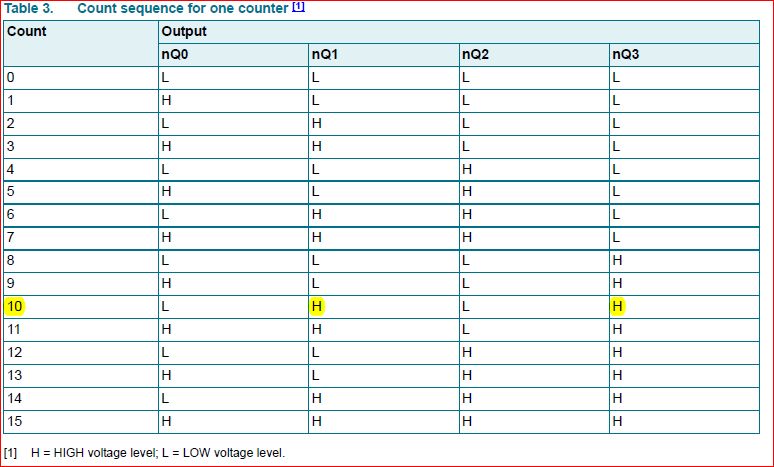
\includegraphics[height=5cm]{../Hardware/Flow_Sensor/Screenshots/FS_logicTable}
	\caption{74HC393 logic}
	\label{screenshot:logicTable}
\end{figure}

Ved praktiske målinger forventes en $PWM_{max}=40-50Hz$.
Det giver systemet som maximum 80ms til at reset'e counteren inden en potentiel fejltriggering.

\begin{figure}[H]
    \begin{align*}
       \frac{1}{frekvens[Hz]} &= Periodetid[ms] \\
       \frac{1}{50[Hz]} &= 20[ms] \\
       4[clockcycles]*20[ms] &= 80[ms] \\ 
    \end{align*}
\label{eq:Trigger}
\caption{Beregning af trigger}
\end{figure}

Simulering af Counter-timing ses på  \ref{screenshot:counterTiming} herunder.

\begin{figure}[H]
	\centering
	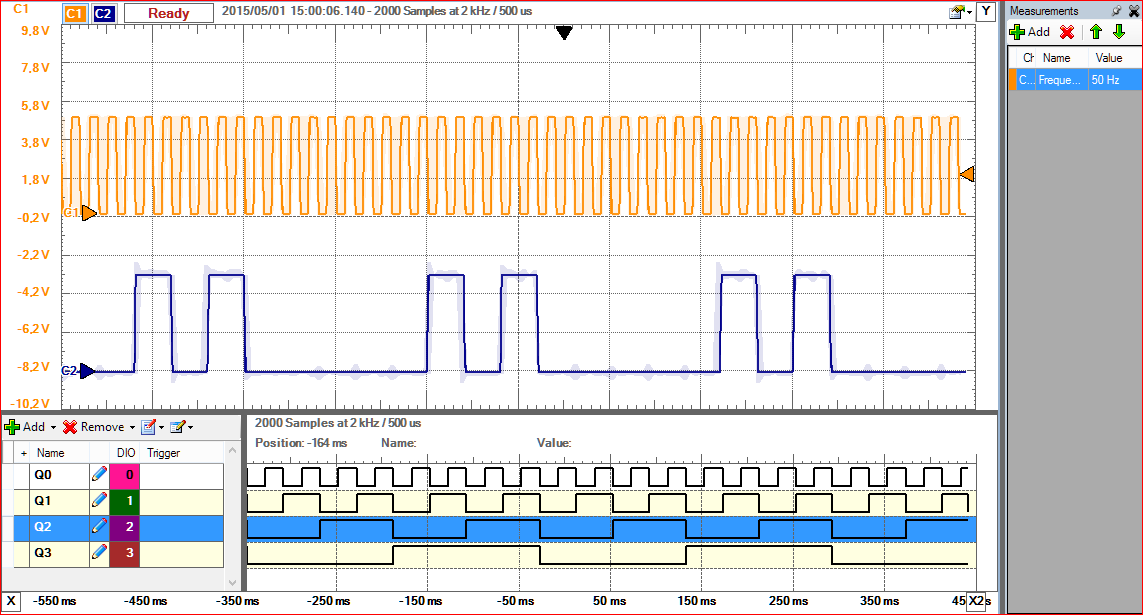
\includegraphics[height=7cm]{../Hardware/Flow_Sensor/Screenshots/FlowSensor_Timingsdiagram}
	\caption{Counter-Timingsdiagram}
	\label{screenshot:counterTiming}
\end{figure}

Denne opsætning med ekstern counter, kan kun lade sig gøre fordi der ikke behøves en ultra præcis måling af vandflowet. 
Ved at lave INT hver 10 gang, midles der over vandflowet. 
Dokumentation til flowsensor-softwarestyring findes under "Software-afsnittet".
